%%%%%%%%%%%%%%%%%%%%%%%%%%%%%%%%%%%%%%%%%
% Journal Article
% LaTeX Template
% Version 1.4 (15/5/16)
%
% This template has been downloaded from:
% http://www.LaTeXTemplates.com
%
% Original author:
% Frits Wenneker (http://www.howtotex.com) with extensive modifications by
% Vel (vel@LaTeXTemplates.com)
%
% License:
% CC BY-NC-SA 3.0 (http://creativecommons.org/licenses/by-nc-sa/3.0/)
%
%%%%%%%%%%%%%%%%%%%%%%%%%%%%%%%%%%%%%%%%%

%----------------------------------------------------------------------------------------
%	PACKAGES AND OTHER DOCUMENT CONFIGURATIONS
%----------------------------------------------------------------------------------------

\documentclass[twoside]{article}

\usepackage{blindtext} % Package to generate dummy text throughout this template 

\usepackage[sc]{mathpazo} % Use the Palatino font
\usepackage[T1]{fontenc} % Use 8-bit encoding that has 256 glyphs
\linespread{1.05} % Line spacing - Palatino needs more space between lines
\usepackage{microtype} % Slightly tweak font spacing for aesthetics

\usepackage[english]{babel} % Language hyphenation and typographical rules

\usepackage[hmarginratio=1:1,top=32mm,columnsep=20pt]{geometry} % Document margins
\usepackage[hang, small,labelfont=bf,up,textfont=it,up]{caption} % Custom captions under/above floats in tables or figures
\usepackage{booktabs} % Horizontal rules in tables

\usepackage{lettrine} % The lettrine is the first enlarged letter at the beginning of the text

\usepackage{enumitem} % Customized lists
\setlist[itemize]{noitemsep} % Make itemize lists more compact

\usepackage{abstract} % Allows abstract customization
\renewcommand{\abstractnamefont}{\normalfont\bfseries} % Set the "Abstract" text to bold
\renewcommand{\abstracttextfont}{\normalfont\small\itshape} % Set the abstract itself to small italic text

\usepackage{titlesec} % Allows customization of titles
\renewcommand\thesection{\Roman{section}} % Roman numerals for the sections
\renewcommand\thesubsection{\roman{subsection}} % roman numerals for subsections
\titleformat{\section}[block]{\large\scshape\centering}{\thesection.}{1em}{} % Change the look of the section titles
\titleformat{\subsection}[block]{\large}{\thesubsection.}{1em}{} % Change the look of the section titles

\usepackage{fancyhdr} % Headers and footers
\pagestyle{fancy} % All pages have headers and footers
\fancyhead{} % Blank out the default header
\fancyfoot{} % Blank out the default footer
\fancyhead[C]{Running title $\bullet$ May 2016 $\bullet$ Vol. XXI, No. 1} % Custom header text
\fancyfoot[RO,LE]{\thepage} % Custom footer text

\usepackage{titling} % Customizing the title section

% My packages (not template)
\usepackage{hyperref} % For hyperlinks in the PDF
%\usepackage{amsmath}
\usepackage{amssymb}
\usepackage{authblk}
\usepackage{graphicx}
\graphicspath{ {figures_report/} }

% From mortens LaTex file:
\usepackage{amsfonts, amssymb, amsmath}
\newcommand{\md}{\mathrm{d}}
\newcommand{\e}[1]{\times 10^{#1}}
\newcommand{\bra}[1]{\langle #1 |}
\newcommand{\ket}[1]{| #1 \rangle}
\newcommand{\braket}[2]{\langle #1 | #2 \rangle}
\renewcommand{\vec}[1]{\mathbf{#1}}
\newcommand{\gvec}[1]{\boldsymbol{#1}}
\newcommand{\dr}{\, \mathrm d^3 \vec r}
\newcommand{\dk}{\, \mathrm d^3 \vec k}

\usepackage{simpler-wick}

%----------------------------------------------------------------------------------------
%	TITLE SECTION
%----------------------------------------------------------------------------------------

\setlength{\droptitle}{-4\baselineskip} % Move the title up

\pretitle{\begin{center}\Huge\bfseries} % Article title formatting
\posttitle{\end{center}} % Article title closing formatting
\title{Building a Shell Model Code: The Pairing Model and the sd-Shell (and comparing results with NuShellX)} % Article title


\author[1]{ \textsc{Gianluca Salvioni}}
\author[2]{ \textsc{Ina K. B. Kullmann}}
\author[3]{ \textsc{Matthew Shelley}}
\author[4]{ \textsc{Gilho Ahn}}


\affil[1]{Department of Physics, University of Jyv\"{a}skyl\"{a},  {\textit {\href{mailto:gianlucasalvioni@gmail.com}{gianlucasalvioni@gmail.com} }}}

\affil[2]{Department of Physics, University of Oslo,  {\textit {\ \href{mailto:i.k.b.kullmann@fys.uio.no}{i.k.b.kullmann@fys.uio.no} }}}

\affil[3] {Department of FILL IN, \LaTeX\ University, \textit {\href{mailto:youremail@edu.com}{youremail@edu.com} }}

\affil[4] {Department of FILL IN, \LaTeX\ University, \textit {\href{mailto:youremail@edu.com}{youremail@edu.com} }}


% another way of doing the authors:
%\author{%
%\textsc{Gianluca Salvioni, Matthew Shelley, Gilho Ahn}\thanks{A thank you} \\[1ex]
%\normalsize University of Oslo \\ % Your institution
%\normalsize \href{mailto:i.k.b.kullmann@fys.uio.no}{i.k.b.kullmann@fys.uio.no} % Your email address
%\and % Uncomment if 2 authors are required, duplicate these 4 lines if more
%\textsc{Ina K. B. Kullmann}\thanks{Corresponding author} \\[1ex] % Second author's name
%\normalsize University of Oslo \\ % Your institution
%\normalsize \href{mailto:i.k.b.kullmann@fys.uio.no}{i.k.b.kullmann@fys.uio.no} % Your email address
%}



\date{\today} % Leave empty to omit a date

\renewcommand{\maketitlehookd}{%
\begin{abstract}

We have first implemented the pairing model which have a analytical solution (to benchmark the code). Then implemented the sd shell ---> more general shell-model program that allows you to study general nuclear structure problems.

developing our own shell-model code that can perform shell-model studies of the oxygen isotopes using standard effective interactions (provided by us) using as example the 1s0d shell as model space.

We have also used the NushellX code in order to perform more advanced shell-model studies and compare the results obtained with your own shell-model code to those of NushellX

and found that.....results...

\end{abstract}
}

%----------------------------------------------------------------------------------------

\begin{document}

% Print the title
\maketitle

%----------------------------------------------------------------------------------------
%	ARTICLE CONTENTS
%----------------------------------------------------------------------------------------

\section{Introduction}

\lettrine[nindent=0em,lines=3]{L} orem ipsum dolor sit amet, consectetur adipiscing elit.
\blindtext % Dummy text

\blindtext % Dummy text

%------------------------------------------------


\section{The pairing problem}

The starting point is a pairing model: the system consists of fermions combined together in pairs of two, one with spin up and one with spin down. The assumption is that the 'breaking of pairs' is not allowed, i.e. the pairs of particles always will be coupled together, forming states with $J$=0. Of consequences the excited states are obtained from the excitation of two particles at the same time. \\
\\
The physics of this system can be described by an Hamiltonian $\hat H$ consisting of an unperturbed one-body operator $\hat H_0$ and a two-body pertubation $\hat V $ defined as 'pairing potential': $\hat H = \hat H_0 + \hat V$. In second quantization we can write:

\begin{equation}
\hat H_0 =  \sum_{p,\sigma} (\epsilon_p-1) \hat a_{p\sigma}^\dagger \hat a_{p\sigma},
\label{eq:H_0}
\end{equation}

\begin{equation}
\hat V = -\frac{1}{2} g \sum_{p,q} \hat a_{p+}^\dagger \hat a_{p-}^\dagger \hat a_{q-} \hat a_{q+} ,\label{eq:V}
\end{equation}
where the fermion creation and annihilation operators are given by $\hat a_{p}^\dagger$ and $\hat a_{q}$ respectively and $pqrs$ represent all possible single-particle quantum numbers.

The single-particle states $\vert p \rangle$ are chosen as eigenfunctions of the one-particle operator $\hat{h}_0$, then the Hamiltonian $H$ acts in turn on various many-body Slater determinants constructed from the single-basis defined by the one-body operator $\hat{h}_0$.

The two-body pairing operator $\hat{V}$ is:
\begin{equation}
\langle q_+ q_- \vert \hat{V} \vert s_+s_- \rangle = -g
\end{equation}
where it is explicitly shown that for a given matrix element $\langle pq \vert \hat{V} \vert rs \rangle$ the states $p$ and $q$ (or $r$ and $s$) must have opposite spin ($\sigma=\pm 1$). $g$ is the (constant) strenght of the pairing interaction.

Using the formalism of second-quantization, the rules of anticommutation for fermions and the products of commutating and anticommutating operators can be shown that $\hat{H}_0$ and $\hat{V}$ commute with the spin projection $\hat{J}_z$ and the total spin $\hat{J}^2$. This means that $H$ can be diagonalized in separated blocks. And due to the 'no-broken pair' assumption, only $J = 0$ are allowed.


\paragraph{Constructing the Hamiltonian matrix}

We are now interested to consider a system consisting of only four particles to calculate its exact analytic solution as benchmark for our shell-model code. The single-particle space is constructed by the four lowest levels with single-particle level energies $\epsilon_p = 1, 2, 3, 4$. Every level $\epsilon_p$ contains two particles, one with spin up $\vert p+ \rangle$ and one with spin down $\vert p- \rangle$. 

The possible Slater determinants that we can build are 6:
\begin{align*}
\ket{\Phi_0} &= \hat a_{2+}^\dagger \hat a_{2-}^\dagger \hat a_{1+}^\dagger \hat a_{1-}^\dagger \ket{0}  \\
%
\ket{\Phi_1} &= \hat a_{3+}^\dagger \hat a_{3-}^\dagger \hat a_{1+}^\dagger \hat a_{1-}^\dagger \ket{0}  \\
%
\ket{\Phi_2} &= \hat a_{4+}^\dagger \hat a_{4-}^\dagger \hat a_{1+}^\dagger \hat a_{1-}^\dagger \ket{0}  \\
%
\ket{\Phi_3} &= \hat a_{3+}^\dagger \hat a_{3-}^\dagger \hat a_{2+}^\dagger \hat a_{2-}^\dagger \ket{0}  \\
%
\ket{\Phi_4} &= \hat a_{4+}^\dagger \hat a_{4-}^\dagger \hat a_{2+}^\dagger \hat a_{2-}^\dagger \ket{0}  \\
%
\ket{\Phi_5} &= \hat a_{4+}^\dagger \hat a_{4-}^\dagger \hat a_{3+}^\dagger \hat a_{3-}^\dagger \ket{0} , \\
\end{align*}

from which we can construct the basis for the Hamiltonian matrix:
\[ \ket{\Phi_0} = \begin{pmatrix} 1 \\ 0 \\ 0 \\ 0 \\ 0 \\ 0 \end{pmatrix}, \quad
\ket{\Phi_1} = \begin{pmatrix} 0 \\ 1 \\ 0 \\ 0 \\ 0 \\ 0 \end{pmatrix}, \quad \cdots \quad
\ket{\Phi_5} = \begin{pmatrix} 0 \\ 0 \\ 0 \\ 0 \\ 0 \\ 1 \end{pmatrix}. \]

The matrix elements $H_{ij}=\bra{\Phi_i} \hat H \ket{\Phi_j}$ \footnote{We use the label 0 to indicate the Slater determinants with the 4 particles in the lowest states, then the first row first column matrix element is $H_{00}$....} are obtained using the Hamiltonian of Eq.~\eqref{eq:H_0}, the Slater determinants and the Wick-theorem. $\hat H_0$ acts only on the diagonal and results in terms proportional with $(\epsilon_p-1)$. The interaction will excite or deexcite a pair of particles from level $q$ to level $p$. \\Using the Wick-theorem, we notice that only the Slater determinants that differ for maximum a pair can interact among them through the pairing potential:
\begin{eqnarray}\label{Vwick}
\bra{\Phi_i} \hat V \ket{\Phi_j} &=&  \bra{0} \hat a_{i_1-} \hat a_{i_1+} \hat a_{i_2-} \hat a_{i_2+} \left[ -\frac{1}{2} g \sum_{p,q} \hat a_{p+}^\dagger \hat a_{p-}^\dagger \hat a_{q-} \hat a_{q+} \right] \hat a_{j_2+}^\dagger \hat a_{j_2-}^\dagger \hat a_{j_1+}^\dagger \hat a_{j_1-}^\dagger \ket{0} \nonumber \\
&=& -\frac{1}{2} g  \left(\delta_{p, i_2} \delta_{q, j_2} \delta_{i_1,j_1} + 
\delta_{p, i_2} \delta_{q, j_1} \delta_{i_1,j_2} + 
\delta_{p, i_1} \delta_{q, j_2} \delta_{i_2,j_1} +
\delta_{p, i_1} \delta_{q, j_1} \delta_{i_2,j_2} \right) 
\end{eqnarray}

and Eq.(\ref{Vwick}) is not null only if at least one of $\delta_{i_1,j_1}, \delta_{i_1,j_2}, \delta_{i_2,j_1}$ or $\delta_{i_2,j_2}$ among bra and ket states is not zero.\\
For example the first term in Eq.(\ref{Vwick}) is obtained from the contractions

\begin{equation}
 \bra{0} \wick{  \c1{\hat a_{i_1-}} \c2{\hat a_{i_1+}} \c3{\hat a_{i_2-}} \c4{\hat a_{i_2+}} \c4{\hat a_{p+}^\dagger} \c3{\hat a_{p-}^\dagger} \c5{\hat a_{q-}} \c6{\hat a_{q+}} \c6{\hat a_{j_2+}^\dagger} \c5{\hat a_{j_2-}^\dagger} \c2{\hat a_{j_1+}^\dagger} \c1{\hat a_{j_1-}^\dagger}} \ket{0} = \delta_{p, i_2} \delta_{q, j_2} \delta_{i_1,j_1}. \nonumber
\end{equation}
 
 Explicitly, the matrix element $H_{00}$ is
\begin{eqnarray}
\bra{\Phi_0} \hat H \ket{\Phi_0} &=& \bra{0} \hat a_{1-} \hat a_{1+} \hat a_{2-} \hat a_{2+} \left[ \sum_{p,\sigma} (\epsilon_p-1) \hat a_{p\sigma}^\dagger \hat a_{p\sigma} \right] \hat a_{2+}^\dagger \hat a_{2-}^\dagger \hat a_{1+}^\dagger \hat a_{1-}^\dagger \ket{0} \nonumber \\
&+& \bra{0} \hat a_{1-} \hat a_{1+} \hat a_{2-} \hat a_{2+} \left[ -\frac{1}{2} g \sum_{p,q} \hat a_{p+}^\dagger \hat a_{p-}^\dagger \hat a_{q-} \hat a_{q+} \right] \hat a_{2+}^\dagger \hat a_{2-}^\dagger \hat a_{1+}^\dagger \hat a_{1-}^\dagger \ket{0} \nonumber \\
&=& 2 \cdot 0+2 \cdot (2-1)+ 2\cdot \left(-\frac{1}{2} g \right) = 2-g.
\end{eqnarray}

The Hamiltonian matrix becomes

\begin{equation}
\hat H = \begin{pmatrix}
2 - g & -g/2 & -g/2 & -g/2 & -g/2 & 0 \\
-g/2 & 4- g & -g/2 & -g/2 & 0 & -g/2 \\
-g/2 & -g/2 & 6 -g & 0 & -g/2 & -g/2 \\
-g/2 & -g/2 & 0 & 6 -g & -g/2 & -g/2 \\
-g/2 & 0 & -g/2 & -g/2 & 8 - g & -g/2 \\
0 & -g/2 & -g/2 & -g/2 & -g/2 & 10 - g \\
\end{pmatrix} .
\label{eq: analytic_H_matrix} 
\end{equation}

\begin{figure}[ht]
\centering
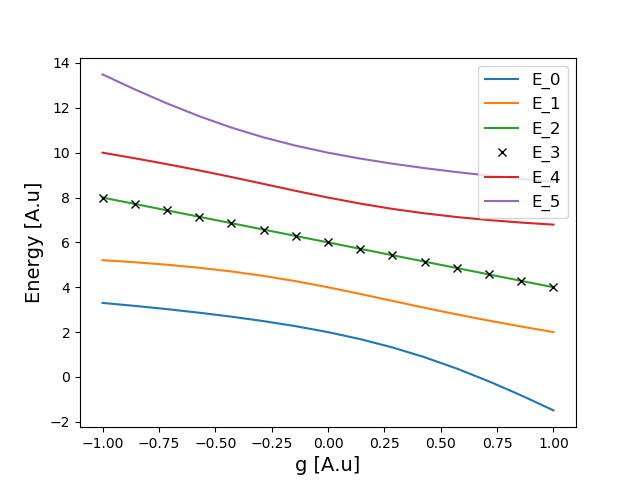
\includegraphics[width=0.8\textwidth]{eigval_vs_g.png}
\caption{The energy levels as a function of the strength $g$ for the analytic case of the pairing model. }
\label{fig: g_vs_eigval}
\end{figure}

In Figure \ref{fig: g_vs_eigval} we see the eigenvalues of the Hamiltonian matrix \eqref{eq: analytic_H_matrix} for the pairing model as a function of the strength $g \in [-1,1]$. \footnote{The diagonalization was done with numpy}.

We can observe that the pairing potential increases the gap among the energy levels $E\_i$, eigenvalues of Eq.(\ref{eq: analytic_H_matrix}). The case $g=1$, corresponding to a strong attractive pairing, produces the more stable system (lowest energy levels).


%------------------------------------------------


\section{Building the shell model code}

develop a code which sets up the above Hamiltonian matrices for two and four particles in 2 and 4 single-particles states (the same as what you did in exercises b) and c) and obtain the eigenvalues.

What did we choose?
\begin{itemize}
\item Decide whether you want to read from file the single-particle data and the matrix elements in m-scheme, or set them up internally in your code. The latter is the simplest possibility for the pairing model, whereas the first option gives you a more general code which can be extended to the more realistic cases discussed in the second part.
\item Based on the single-particle basis, write a function which sets up all possible Slater determinants which have total M = 0. Test that this function reproduces the cases in b) and c). If you make this function more general, it can then be reused for say a shell-model calculation of sd-shell nuclei in the second part.
\item Use the Slater determinant basis from the previous step to set up the Hamiltonian matrix.
\item With the Hamiltonian matrix, you can finally diagonalize the matrix and obtain the final eigenvalues and test against the results of b) and c).
\end{itemize}

Include some of this? Or too much? :\\
The lecture slides contain a rather detailed recipe on how to construct a Slater determinant basis and how to set up the Hamiltonian matrix to diagonalize.



\subsection{first step....}

\subsection{Unit tests and benchmarks}

(have not done this?)

One obvious case is that of removing the two-body interaction. Then we have only the single-particle energies. For the case of degenerate single-particle orbits, that is one value of total single-particle angular momentum only $j$, with degeneracy $\Omega = 2j + 1$, one can show that the ground state energy $E_0$ is with $n$ particles

\begin{equation}
E_0 = -\frac{g}{4}n (\Omega - n + 2)
\end{equation}

Enlarge now your system to six and eight fermions and to $p = 6$ and $p = 8$ single-particle states, respectively. Run your program for a degenerate single-particle state with degeneracy $\Omega$ and test against the exact result for the ground state. Introduce thereafter a finite single-particle spacing and study the results as you vary $g$, as done in b) and c). Comment your results.

(describe the unit test that we have implemented and how)


%------------------------------------------------


\section{NuShellX}
(describe what is, then put results in results section?)


\section{Results}

%\begin{table}
%\caption{Example table}
%\centering
%\begin{tabular}{llr}
%\toprule
%\multicolumn{2}{c}{Name} \\
%\cmidrule(r){1-2}
%First name & Last Name & Grade \\
%\midrule
%John & Doe & $7.5$ \\
%Richard & Miles & $2$ \\
%\bottomrule
%\end{tabular}
%\end{table}




%------------------------------------------------

\section{Discussion}


%------------------------------------------------


\section{Conclusions}



%------------------------------------------------



\section*{Structure of report (crude first idea):}

\begin{enumerate}
\item Title
\item Abstract
\item Introduction
\begin{itemize}
\item Why useful
\item Where useful (nuc. chart)
\item (Look at the TALENT proposal)
\item comparing different tools
\end{itemize}
\item The Pairing problem
\begin{itemize}
\item theory
\item analytic / exact results
\end{itemize}
\item Building a shell-model code
\begin{itemize}
\item Describe the different parts/blocks of the code (basis, SD, states, int, hamiltonian...)
\item Unit tests / benchmarks (analytic/exact results)
\item Psedo code?
\item Accuracy of our code
\item Where our code fails, why and proposing solutions
\end{itemize}
\item NuShellX
\begin{itemize}
\item describe why useful / 'powerful tool' and what may be calculated
\item compare with our own code
\item Possible 'future calculations'
\end{itemize}
\item Conclusions / Summary
\end{enumerate}

%------------------------------------------------
%------------------------------------------------




%----------------------------------------------------------------------------------------
%	REFERENCE LIST
%----------------------------------------------------------------------------------------

\begin{thebibliography}{99} % Bibliography - this is intentionally simple in this template
%
%\bibitem[Figueredo and Wolf, 2009]{Figueredo:2009dg}
%Figueredo, A.~J. and Wolf, P. S.~A. (2009).
%\newblock Assortative pairing and life history strategy - a cross-cultural
%  study.
%\newblock {\em Human Nature}, 20:317--330.

\bibitem[Github of the TALENT School][ MHJ and Alex Brown
\newblock {\em link goes here},
 
\end{thebibliography}

%----------------------------------------------------------------------------------------

\end{document}
